\documentclass[a4paper,11pt]{report}

\usepackage[utf8]{inputenc}
\usepackage[T1]{fontenc}
\usepackage[francais]{babel}

\usepackage{graphicx}
\usepackage{tabularx}

\title{Evalens -- Analyse}
\date{}

\begin{document}
\maketitle
\tableofcontents

\chapter{Lexique}

\subsection{Doyen}

\subsection{Gestionnaire de campagne}
Entité pouvant être composée de plusieurs personnes.

\subsection{Commision pédagogique facultaire}
\subsubsection{Membre}
\subsubsection{Président}

\subsection{Étudiant}

\subsection{Enseignant}

\subsection{Cellule de communication universitaire}

\subsection{Unité d'enseignement}

\subsection{Calendrier}

\subsection{Période}
Intervalle de temps ayant une date et une heure de début et de fin.

\chapter{Cas d'utilisation}
\begin{figure}[ht]
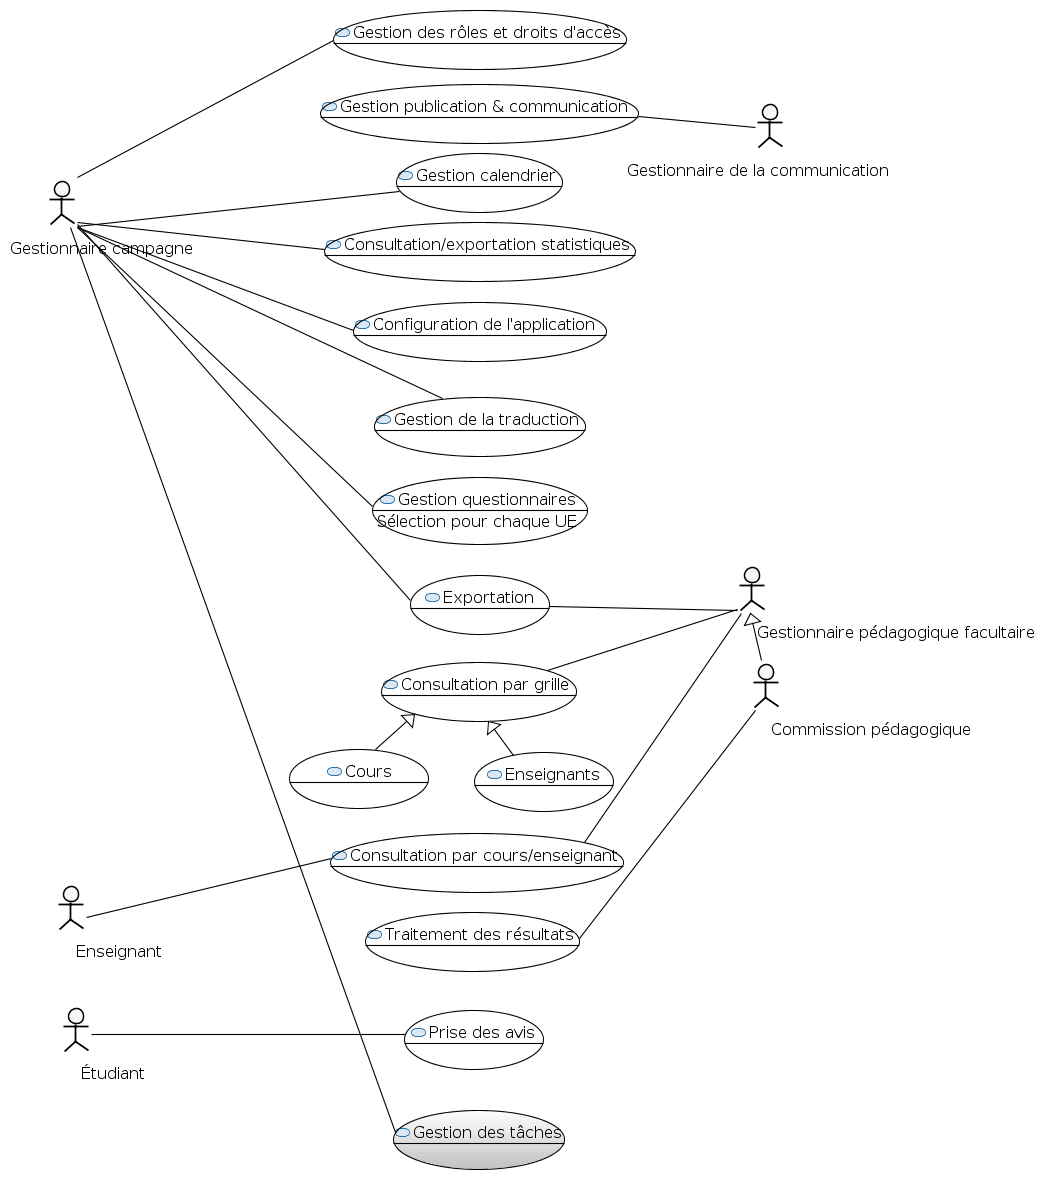
\includegraphics[width=\linewidth]{UseCase_Diagram.PNG}
\caption{Diagramme des cas d'utilisation}
\label{fig:usecase-diag}
\end{figure}

\section{Évaluation des enseignements}

\subsection{Gestion des rôles et des droits d'accès}
Chaque utilisateur a un rôle et des droits d'accès différents.

\begin{table}[ht]
\begin{tabularx}{\textwidth}{|X|l|} \hline
Rôle & Droits d'accès \\ \hline
Gestionnaire des rôles et droits d'accès & \\ \hline
Gestionnaire des publications et de la communication & \\ \hline
Configuration de l'application & \\ \hline
Gestionnaire de la traduction & \\ \hline
Gestionnaire des questionnaires & \\ \hline
DAF & \\ \hline
Président de la com péd & \\ \hline

\end{tabularx}
\caption{Rôle et droits d'accès des différents utilisateurs du système. «~com. péd.~» est l'abbréviation de «~commission pédagogique~».}
\label{tab:role-droit}
\end{table}

Certains rôles et droits d'accès peuvent être amenés à évoluer, et d'autres pourraient être ajoutés par la suite.

\subsection{Gestion des publications et de la communication}
Le gestionnaire de campagne est chargé de communiquer l'état de la campagne aux acteurs concernés~; l'ouverture de la prise d'avis est annoncée aux étudiants, la disponibilité des résultats aux enseignants.\footnote{Quelle est la liste exhaustive des informations à communiquer et quand ? Dans le calendrier ?}

Texte pouvant être modifié sur base d'un modèle.

Publication : pdf à mettre à diposition d'autres systèmes/personnes

\subsection{Gestion du calendrier}
La gestion du calendrier est une étape nécessaire à une campagne~; elle permet de définir les périodes de validité de certaines activités ainsi que les dates de planification des tâches, potentiellement par faculté.
Cette gestion permet de déclarer une période de suspension pour toute période définie en cas de besoin.

\noindent Elle est prise en charge par le gestionnaire de campagne.

\noindent Parmi ces dates et périodes, on trouve~:
\begin{itemize}
	\item Invitation à la prise d'avis~: date et heure à laquelle le mail d'invitation à la prise d'avis est envoyé aux étudiants.
	\item Rappel à la prise d'avis~: date et heure à laquelle le mail de rappel de prise d'avis est envoyé aux participants qui n'ont pas rempli certains critères (exemple~: participants ayant répondu à moins de 80~\% des questions).
	\item Prise d'avis~: période durant laquelle les étudiants ont accès aux questionnaires et peuvent les remplir.
	\item Traitement des résultats~: période durant laquelle la commission pédagogique a accès au traitement des résultats. La commission a aussi l'opportunité de consulter les résultats à partir du début de cette période, dès lors que le traitement est terminé.
	\item Consultation des résultats par les enseignants~: date à partir de laquelle les enseignants ont accès aux résultats de la campagne.
	\item Consultation des résultats par grille~: date à partir de laquelle les résultats par grille sont accessibles par un ensemble de rôle.
\end{itemize}
~\newline{}

La constitution du calendrier est régie par les règles et contraintes suivantes~:
\begin{itemize}
	\item Chaque date et période déclarée doit être liée à une campagne.
	\item La période de prise d'avis doit être incluse dans la période de la campagne.
	\item La date d'invitation des prises d'avis doit être entérieure à la date de début de la période de prise d'avis.
	\item La date de rappel à la prise d'avis doit être incluse dans la période de prise d'avis.
	\item Le traitement des résultats est suspendu tant qu'une période de prise d'avis est en cours.
	\item La date de consultation des résultats par les enseignants doit être postérieure à la date de fin de la période de traitement des résultats.
\end{itemize}


\subsection{Configuration de l'application}

\subsection{Gestion de la traduction}
L'ensemble des questions et de l'interface doit pouvoir être traduit dans une autre langue que le français.

\subsection{Gestion des questionnaires}
Lors de chaque campagne, un questionnaire est associé à chaque unité d'enseignement.
Ce questionnaire peut changer d'une campagne à l'autre, mais il doit être possible de retrouver celui correspondant à une campagne donnée.

\subsection{Exportation}
Les différentes données accessibles à l'utilisateur doivent pouvoir être exportées en différents formats~:
\begin{itemize}
	\item CSV
	\item PDF
\end{itemize}



\subsection{Consultation des résultats par grilles des cours}

\subsection{Consultation des résultats par grilles des enseignants}

\subsection{Consultation par cours/enseignant}
Les enseignants ont la possibilité de consulter leurs résultats de deux façons différentes~:
\begin{itemize}
	\item en vue globale rassemblant toutes leurs unités d'enseignement~;
	\item une unité d'enseignement à la fois.
\end{itemize}

Les titulaires des unités d'enseignement peuvent consulter

\subsection{Traitement des résultats}

\subsection{Prise des avis}
Enregistrement des avis entrés par les étudiants.

\end{document}